\documentclass{article}
\usepackage[english]{babel}
\usepackage{amsmath,amssymb,graphicx,bbm,hyperref,latexsym,theorem}
\usepackage{mathtools}

\numberwithin{equation}{section}

%%%%%%%%%% Start TeXmacs macros
\catcode`\<=\active \def<{
\fontencoding{T1}\selectfont\symbol{60}\fontencoding{\encodingdefault}}
\newcommand{\assign}{:=}
\newcommand{\comma}{{,}}
\newcommand{\nin}{\not\in}
\newcommand{\tmdummy}{$\mbox{}$}
\newcommand{\tmop}[1]{\ensuremath{\operatorname{#1}}}
\newcommand{\tmscript}[1]{\text{\scriptsize{$#1$}}}
\newcommand{\tmtextbf}[1]{{\bfseries{#1}}}
\newcommand{\tmtextit}[1]{{\itshape{#1}}}
\newcommand{\tmtextmd}[1]{{\mdseries{#1}}}
\newcommand{\tmtextrm}[1]{{\rmfamily{#1}}}
\newcommand{\tmtextup}[1]{{\upshape{#1}}}
\newenvironment{proof*}[1]{\noindent\textbf{#1\ }}{\hspace*{\fill}$\Box$\medskip}
\newtheorem{corollary}{Corollary}[section]
{\theorembodyfont{\rmfamily}\newtheorem{example}[corollary]{Example}}
\newtheorem{lemma}[corollary]{Lemma}
\newtheorem{proposition}[corollary]{Proposition}
{\theorembodyfont{\rmfamily}\newtheorem{remark}[corollary]{Remark}}
\newtheorem{theorem}[corollary]{Theorem}
%%%%%%%%%% End TeXmacs macros

%proofreading symbols
\newcommand{\mykana}[2]{#1}
\newcommand{\doubt}[1]{\fbox{#1}}
\newcommand{\pause}{$\bullet$}
\newcommand{\slowly}[1]{\dashuline{#1}}
\newcommand{\continuously}[1]{\underline{#1}}
\newcommand{\badword}[1]{\uwave{#1}}

%my commants
\newcommand{\mygrammarfootnote}[1]{}

\newcommand{\sectionsep}{{\sectionalsep}}

\begin{document}

September 19, 2017

\begin{abstract}
  Motivated by the study of symmetry breaking operators for indefinite
  orthogonal groups, we give a Gegenbauer expansion of the two variable
  function $| s + t |^{\alpha}$ in terms of the ultraspherical polynomials
  $C_{\ell}^{\lambda} (s)$ and $C^{\mu}_m (t)$.
  
  Specializations and limits of the expansion are discussed in the context of
  specializations of the Selberg integral and its
  generalization\mygrammarfootnote{maybe, ``generalization'' should be in plural (i.e.
  ``generalizations'')?} by Dotsenko, Fateev, Tarasov, Varchenko, and Warnaar
  among others.
\end{abstract}

\section{Main results}

\begin{theorem}
  For $\lambda, \mu, \nu \in \mathbbm{C}$ with $\tmop{Re} \lambda, \tmop{Re}
  \mu, \tmop{Re} \nu > - 1 / 2$, \ the following expansion holds:
  \begin{eqnarray}
    & | s + t |^{2 \nu} = \sum_{\ell, m = 0 \mid \ell + m :
    \tmop{even}}^{\infty} a_{\lambda, \mu, \nu}^{\ell, m} C_{\ell}^{\lambda}
    (s) C_m^{\mu} (t), &  \nonumber\\
    & a_{\lambda, \mu, \nu}^{\ell, m} = \frac{2^{- 2 \nu} (\lambda + \ell)
    (\mu + m) \Gamma (\lambda + \mu + 2 \nu + 1) \Gamma (\lambda) \Gamma (\mu)
    \Gamma (2 \nu + 1)}{\Gamma \left( \lambda + \nu + \frac{\ell - m}{2} + 1
    \right) \Gamma \left( \mu + \nu - \frac{\ell - m}{2} + 1 \right) \Gamma
    \left( \lambda + \mu + \nu + \frac{\ell + m}{2} + 1 \right) \Gamma \left(
    \nu + 1 - \frac{\ell + m}{2} \right)} . &  \nonumber
  \end{eqnarray}
\end{theorem}

Let $C_{\ell}^{\lambda} (s)$ be the Gegenbauer polynomial of degree $\ell$,
and we set
\[ u_{\ell}^{\lambda} (s) \assign \frac{2^{2 \lambda - 1} \ell ! \Gamma
   (\lambda)}{\Gamma (2 \lambda + \ell)} (1 - s^2)^{\lambda - \frac{1}{2}}
   C_{\ell}^{\lambda} (s) . \]
\begin{theorem}
  \label{main-thm}Suppose $\ell, m \in \mathbbm{N}$ such that $\ell + m$ is
  even. For $\lambda, \mu, \nu \in \mathbbm{C}$ with $\tmop{Re} \lambda,
  \tmop{Re} \mu, \tmop{Re} \nu > - 1 / 2$, and for $- 1 \leqslant x \leqslant
  1$, \ the following integral converges:
  \begin{eqnarray}
    & \displaystyle\int_{- 1}^1 \displaystyle\int_{- 1}^1 | s + t x |^{2 \nu} u_{\ell}^{\lambda} (s)
    u_m^{\mu} (t) d s d t &  \nonumber\\
    & = \frac{(- \nu)_{\frac{\ell + m}{2}} (- 1)^{\frac{\ell + m}{2}}
    \pi^{\frac{3}{2}} \Gamma \left( \nu + \frac{1}{2} \right) x^m _2 F_1
    \left( \begin{array}{c}
      \frac{\ell + m}{2} - \nu, \frac{m - \ell}{2} - \nu - \lambda\\
      \mu + m + 1
    \end{array} ; x^2 \right)}{\Gamma (\mu + m + 1) \Gamma \left( \lambda +
    \nu + \frac{\ell - m}{2} + 1 \right)},  \label{eqn:main} & 
  \end{eqnarray}
  where $(y)_j \assign y (y + 1) (y + 2) \cdots (y + j - 1)$ for $j \in
  \mathbbm{N}$.
\end{theorem}

Note that as the Gegenbauer polynomial $g (s) \assign C_{\ell}^{\lambda} (s)$
satisfies the second-order differential equation
\begin{eqnarray}
  & (1 - s^2) g'' - (2 \lambda + 1) s g' + n (n + 2 \lambda) g = 0, & 
  \nonumber
\end{eqnarray}
$f (s) \assign u_{\ell}^{\lambda} (s)$ satisfies
\begin{eqnarray}
  & (1 - s^2)^2 f'' + (1 - s^2) (1 - 2 \lambda - (2 \lambda + 1) s) f' + ((2
  s + 1) (\lambda^2 - 1 / 4) + \ell (\ell + 2 \lambda) (1 - s^2)) f = 0. & 
  \nonumber
\end{eqnarray}
\begin{remark}
  Since $u_m^{\mu} (- t) = (- 1)^m u_m^{\mu} (t)$, Theorem \ref{main-thm} is
  reduced to the case $0 \leqslant x \leqslant 1$.
\end{remark}

The substitution of $x = 1$ in Theorem \ref{main-thm} yields:

\begin{corollary}
  \label{cor:1}{\tmdummy}
  
  \begin{eqnarray}
    & \displaystyle\int_{- 1}^1 \displaystyle\int_{- 1}^1 | s + t |^{2 \nu} (1 - s^2)^{\lambda -
    \frac{1}{2}} (1 - t^2)^{\mu - \frac{1}{2}} C_{\ell}^{\lambda} (s)
    C_m^{\mu} (t) d s d t &  \nonumber\\
    & = \frac{(- \nu)_{\frac{\ell + m}{2}} (- 1)^{\frac{\ell + m}{2}}
    \pi^{\frac{1}{2}} (2 \lambda)_{\ell} (2 \mu)_m \Gamma \left( \lambda +
    \frac{1}{2} \right) \Gamma \left( \mu + \frac{1}{2} \right) \Gamma \left(
    \nu + \frac{1}{2} \right) \Gamma (\lambda + \mu + 2 \nu + 1)}{\ell !m!
    \Gamma \left( \lambda + \nu + \frac{\ell - m}{2} + 1 \right) \Gamma \left(
    \mu + \nu - \frac{\ell - m}{2} + 1 \right) \Gamma \left( \lambda + \mu +
    \nu + \frac{\ell + m}{2} + 1 \right)}  \label{eqn:cor:1} . & 
  \end{eqnarray}
\end{corollary}

Taking the limit in $(\ref{eqn:cor:1})$ as both $\lambda$ and
$\mu$ tend to be
zero, we obtain

\begin{corollary}
  \label{cor:170599}For $\rho \in \mathbbm{C}$ with $\tmop{Re} \rho > 0$ and
  $r \in \{ 0, 1 \}$,
  \begin{eqnarray}
    & | \cos \varphi + \cos \psi |^{\rho} \tmop{sgn}^r (\cos \varphi + \cos
    \psi) &  \nonumber\\
    & = \sum_{\tmscript{\begin{array}{c}
      \ell, m = 0\\
      \ell \equiv m + r \tmop{mod} 2
    \end{array}}}^{\infty} \frac{2^{2 - \rho} \Gamma (\rho + 1)^2}{(1 +
    \delta_0^{\ell}) (1 + \delta_0^m) \prod_{\delta, \varepsilon \in \{ \pm 1
    \}} \Gamma \left( 1 + \frac{1}{2} (\rho + \delta \ell + \varepsilon m)
    \right)} \cos \ell \varphi \cos m \psi . &  \nonumber
  \end{eqnarray}
  where
  $\delta_0^\ell$ denotes the Kronecker delta, i.e.,
  $\delta_0^{\ell} \assign 1$ if $\ell = 0$ and $= 0$ otherwise.
\end{corollary}

Selberg-type integrals are related to (finite-dimensional) representation
theory of semisimple Lie algebras, see {\cite{forrester2008importance}},
{\cite{tarasov2003selberg}} and references therein. On the other hand, Theorem
\ref{main-thm} and Corollary \ref{cor:1} will be used in the study of symmetry
breaking operators for infinite-dimensional representations when we extend the
work {\cite{kobayashi2015symmetry}} to indefinite orthogonal groups $O (p,
q)$. This will be done in a separate paper.

Special cases and the limit case of Theorem \ref{main-thm} will be discussed
in Section \ref{sec:4}.

\section{Proof of main theorem}\label{sec:2}

In this section we prove Theorem \ref{main-thm} by assuming the following
integral formula $(\ref{eqn:stz})$, which will be proved in Section
\ref{sec:3}.

\begin{proposition}
  \label{prop:2}For $a, b, c \in \mathbbm{C}$ such that $\tmop{Re} a,
  \tmop{Re} b, \tmop{Re} c > 0$ and for $- 1 \leqslant x \leqslant 1$, we have
  \begin{eqnarray}
    & \displaystyle\int_{- 1}^1 \displaystyle\int_{- 1}^1 | s + t x |^{2 c - 1} (1 - s^2)^{a - 1} (1 -
    t^2)^{b - 1} d s d t = \frac{\sqrt{\pi} \Gamma (a) \Gamma (b) \Gamma
    (c)}{\Gamma (a + c) \Gamma \left( b + \frac{1}{2} \right)} _2 F_1 \left(
    \begin{array}{c}
      - c + \frac{1}{2}, - a - c + 1\\
      b + \frac{1}{2}
    \end{array} ; x^2 \right) .  \label{eqn:stz} & \\
    &  &  \nonumber
  \end{eqnarray}
\end{proposition}

\begin{proof*}{Proof of Theorem \ref{main-thm}}
  The Rodrigues formula for the Gegenbauer polynomial (see
  {\cite[(6.4.14)]{andrews2000special}} for instance) shows
  \begin{equation} u_{\ell}^{\lambda} (t) = \frac{(- 1)^{\ell} 2^{- \ell} \sqrt{\pi}}{\Gamma
     \left( \lambda + \ell + \frac{1}{2} \right)} \cdot \frac{d^{\ell}}{d
     t^{\ell}} (1 - t^2)^{\lambda + \ell - \frac{1}{2}} . 
     \label{eqn:Rod} \end{equation}
  Then\mygrammarfootnote{maybe, we need a comma here?} the left-hand side of
  $(\ref{eqn:main})$ amounts to
  \begin{eqnarray}
    & \frac{2^{- \ell - m} \pi}{\Gamma \left( \lambda + \ell + \frac{1}{2}
    \right) \Gamma \left( \mu + m + \frac{1}{2} \right)} I_{\ell, m} (x), & 
    \nonumber
  \end{eqnarray}
  where we set
  \[ I_{\ell, m} (x) \assign \displaystyle\int_{- 1}^1 \displaystyle\int_{- 1}^1 | s + tx |^{2 \nu}
     \frac{\partial^{\ell}}{\partial s^{\ell}} (1 - s^2)^{\lambda + \ell -
     \frac{1}{2}} \frac{\partial^m}{\partial t^m} (1 - t^2)^{\mu + m -
     \frac{1}{2}} d s d t. \]
  Suppose that $\tmop{Re} \nu > \frac{\ell + m}{2}$, $\tmop{Re} \lambda >
  \frac{1}{2}$ and $\tmop{Re} \mu > \frac{1}{2}$. Then $| s + tx |^{2 \nu}$ is
  of $C^{\ell + m}$ class, and integration by parts gives
  \begin{eqnarray}
    & I_{\ell, m} (x) = \displaystyle\int_{- 1}^1 \displaystyle\int_{- 1}^1 (1 - s^2)^{\lambda + \ell -
    \frac{1}{2}} (1 - t^2)^{\mu + m - \frac{1}{2}} \frac{\partial^{\ell +
    m}}{\partial s^{\ell} \partial t^m} | s + t x |^{2 \nu} d s d t. 
    \label{eqn:derst} & 
  \end{eqnarray}
  Since $\ell + m \in 2\mathbbm{N}$ we have
  \[ \frac{\partial^{\ell + m}}{\partial s^{\ell} \partial t^m} | s + tx |^{2
     \nu} = (- 2 \nu)_{\ell + m} x^m | s + t x |^{2 \nu - \ell - m}, \]
  and therefore $(\ref{eqn:derst})$ equals
  \begin{eqnarray}
    & (- 2 \nu)_{\ell + m} x^m \displaystyle\int_{- 1}^1 \displaystyle\int_{- 1}^1 | s + t x |^{2 \nu -
    \ell - m} (1 - s^2)^{\lambda + \ell - \frac{1}{2}} (1 - t^2)^{\mu + m -
    \frac{1}{2}} d s d t. &  \nonumber
  \end{eqnarray}
  Then Theorem \ref{main-thm} follows from Proposition \ref{prop:2} with $(a,
  b, c) = \left( \lambda + \ell + \frac{1}{2}, \mu + m + \frac{1}{2}, \nu +
  \frac{1}{2} (1 - \ell - m) \right)$.
\end{proof*}

\section{Proof of Proposition \ref{prop:2}}\label{sec:3}

In this section we show Proposition \ref{prop:2}, and thus complete the proof
of Theorem \ref{main-thm}. We use the following two lemmas.

\begin{lemma}
  \label{lem4}For $a, b, z \in \mathbbm{C}$ with $\tmop{Re} a, \tmop{Re} b >
  0$ and for $- 1 \leqslant x \leqslant 1$ we have
  \begin{eqnarray}
    & \displaystyle\int_{- 1}^1 (1 + tx)^{a - 1} (1 - t^2)^{b - 1} d t = B \left(
    \frac{1}{2}, b \right) _2 F_1 \left( \begin{array}{c}
      \frac{1 - a}{2}, \frac{2 - a}{2}\\
      b + \frac{1}{2}
    \end{array} ; x^2 \right) . &  \nonumber
  \end{eqnarray}
\end{lemma}

\begin{lemma}
  \label{lem:Fisum}Let $a, b, c \in \mathbbm{C}$ with $b + \frac{1}{2} \nin
  -\mathbbm{N}$. Then\mygrammarfootnote{maybe, we need a comma here?}
  \[ G (a, b, c ; \zeta) \assign \sum_{i = 0}^{\infty} \frac{(a)_i (1 -
     a)_i}{2^i i! (d)_i} _2 F_1 \left( \begin{array}{c}
       \frac{1 - d - i}{2}, \frac{2 - d - i}{2}\\
       b + \frac{1}{2}
     \end{array} ; \zeta \right) \]
  converges when $| \zeta | < 1$, and we have
  \begin{equation} G (a, b, c ; \zeta) = \frac{2^{1 - d} \sqrt{\pi} \Gamma (d)}{\Gamma
     \left( \frac{a + d}{2} \right) \Gamma \left( \frac{1 - a + d}{2} \right)}
     _2 F_1 \left( \begin{array}{c}
       1 - \frac{a + d}{2}, \frac{1 + a - d}{2}\\
       b + \frac{1}{2}
   \end{array} ; \zeta \right) .  \label{eqn:iF}\end{equation}
\end{lemma}

Postponing the verification of Lemmas \ref{lem4} and \ref{lem:Fisum}, we first
show Proposition \ref{prop:2}.

\begin{proof*}{Proof of Proposition \ref{prop:2}}
  By the change of variables $s = 1 - (1 + x) t$, the interval $0 \leqslant t
  \leqslant 1$ is transformed onto $(- 1 \leqslant) - x \leqslant s \leqslant
  1$, and thus Euler's integral representation of the hypergeometric function
  $_2 F_1$ shows
  \begin{eqnarray}
    & \displaystyle\int_{- 1}^1 (s + x)_+^{2 c - 1} (1 - s^2)^{a - 1} d s = 2^{a - 1} B (2
    c, a) (1 + x)^{2 c + a} _2 F_1 \left( \begin{array}{c}
      1 - a, 2 c\\
      2 c + a
    \end{array} ; \frac{1 + x}{2} \right), &  \nonumber
  \end{eqnarray}
  where $y_+^{\lambda} \assign | y |^{\lambda}$ for $y > 0$; $= 0$ for $y
  \leqslant 0$.
  
  Therefore the left-hand side of $(\ref{eqn:stz})$ equals:
  \begin{eqnarray}
    & 2 \displaystyle\int_{- 1}^1 \displaystyle\int_{- 1}^1 (s + tx)_+^{2 c - 1} (1 - s^2)^{a - 1} (1 -
    t^2)^{b - 1} d s d t &  \nonumber\\
    & = 2^a B (2 c, a) \displaystyle\int_{- 1}^1 (1 + tx)^{2 c + a - 1} _2 F_1 \left(
    \begin{array}{c}
      1 - a, a\\
      2 c + a
    \end{array} ; \frac{1 + tx}{2} \right) (1 - t^2)^{b - 1} d t. &  \nonumber
  \end{eqnarray}
  Fix $\varepsilon > 0$. Assume $| x | \leqslant 1 - 2 \varepsilon$. Then
  $\left| \frac{1 + tx}{2} \right| \leqslant 1 - \varepsilon$. Expanding the
  hypergeometric function as a uniformly convergent power series of
  $\frac{1}{2} (1 + tx)$, we can rewrite the integral in the right-hand side
  as
  \begin{eqnarray}
    & \sum_{i = 0}^{\infty} \frac{(1 - a)_i (a)_i}{2^i i! (2 c + a)_i}
    \displaystyle\int_{- 1}^1 (1 + t x)^{2 c + a - 1 + i} (1 - t^2)^{b - 1} d t. & 
    \nonumber
  \end{eqnarray}
  Owing to Lemma \ref{lem4}, this is equal to
  \begin{eqnarray}
    & B \left( \frac{1}{2}, b \right) \sum_{i = 0}^{\infty} \frac{(1 - a)_i
    (a)_i}{2^i i! (2 c + a)_i} _2 F_1 \left( \begin{array}{c}
      \frac{1 - 2 c - a - i}{2}, \frac{2 - 2 c - a - i}{2}\\
      b + \frac{1}{2}
    \end{array} ; x^2 \right) . &  \nonumber
  \end{eqnarray}
  Now (\ref{eqn:stz}) follows from Lemma \ref{lem:Fisum} with $\zeta = z^2$
  and $d = 2 c + a$\mygrammarfootnote{maybe, we need a comma here?} and from the
  duplication formula of the Gamma function $\Gamma (2 c) = \pi^{-
  \frac{1}{2}} 2^{2 c - 1} \Gamma (c) \Gamma \left( c + \frac{1}{2} \right)$.
\end{proof*}

\begin{proof*}{Proof of Lemma \ref{lem4}}
  By Euler's integral representation of $_2 F_1$ again, we have
  \begin{eqnarray}
    & \displaystyle\int_{- 1}^1 (1 - t z)^{a - 1} (1 - t^2)^{b - 1} d t = 2^{2 b - 1} (1 +
    z)^{a - 1} B (b, b)_2 F_1 \left( \begin{array}{c}
      1 - a, b\\
      2 b
    \end{array} ; \frac{2 z}{1 + z} \right) .  \label{eqn:quad} & 
  \end{eqnarray}
  Applying the following quadratic transformation of $_2 F_1$ (cf. {\cite[Thm.
  3.13]{andrews2000special}}):
  \begin{eqnarray}
    & \;_2 F_1 \left( \begin{array}{c}
      1 - a, b\\
      2 b
    \end{array} ; u \right) = \left( 1 - \frac{z}{2} \right)^{a - 1} _2 F_1
    \left( \begin{array}{c}
      \frac{1 - a}{2}, \frac{2 - a}{2}\\
      b + \frac{1}{2}
    \end{array} ; \left( \frac{u}{2 - u} \right)^2 \right), &  \nonumber
  \end{eqnarray}
  with $u = \frac{2 z}{1 + z}$, we get the desired result after a small
  computation using the duplication formula of the $\Gamma$-function.
\end{proof*}

\begin{proof*}{Proof of Lemma \ref{lem:Fisum}}
  We list some elementary identities for the Pochammer symbol $(y)_j =
  \frac{\Gamma (y + j)}{\Gamma (y)}$ satisfies
  \begin{eqnarray}
    & y_j (1 - y)_{- j} & = \; (- 1)^j,  \label{eqn:p1}\\
    & \left( \frac{y}{2} \right)_j \left( \frac{1 + y}{2} \right)_j & = \;
    2^{- 2 j} (y)_{2 j},  \label{eqn:p2}\\
    & (y)_i (1 - y)_{2 j} & = \; (1 - y - i)_{2 j} (y - 2 j)_i . 
    \label{eqn:p3}
  \end{eqnarray}
  We claim that the left-hand side of $(\ref{eqn:iF})$ equals
  \begin{eqnarray}
    & G (a, b, d ; \zeta) = \sum_{j = 0}^{\infty} \frac{(1 - d)_{2 j}
    \zeta^j}{2^{2 j} j! \left( b + \frac{1}{2} \right)_j} _2 F_1 \left(
    \begin{array}{c}
      a, 1 - a\\
      d - 2 j
    \end{array} ; \frac{1}{2} \right) . &  \label{eqn:Fijsum}
  \end{eqnarray}
  Indeed, by expanding the hypergeometric function as a power series and by
  using $(\ref{eqn:p2})$ with $y = 1 - d - i$, we have
  \begin{eqnarray}
    & G (a, b, d ; \zeta) = \sum_{i = 0}^{\infty} \sum_{j = 0}^{\infty}
    \frac{(a)_i (1 - a)_i}{2^{i + 2 j} i!j! (d)_i}  \frac{(1 - d - i)_{2
    j}}{\left( b + \frac{1}{2} \right)_j} \zeta^j, &  \nonumber
  \end{eqnarray}
  which is equal to the right-hand side of $(\ref{eqn:Fijsum})$ by
  $(\ref{eqn:p3})$ with $y = d$. Hence we have verified the equality
  $(\ref{eqn:Fijsum})$.
  
  As $\;_2 F_1 \left( \begin{array}{c}
    a, 1 - a\\
    c
  \end{array} ; \frac{1}{2} \right) = \frac{2^{1 - c} \sqrt{\pi} \Gamma
  (c)}{\Gamma \left( \frac{a + c}{2} \right) \Gamma \left( \frac{c - a + 1}{2}
  \right)}$ (see {\cite[Thm. 5.4]{andrews2000special}} for instance), we can
  continue as
  \begin{eqnarray}
    & \begin{array}{ll}
      (\ref{eqn:Fijsum}) & = \sum_{j = 0}^{\infty} \frac{(1 - d)_{2 j}
      \zeta^j}{2^{2 j} j! \left( b + \frac{1}{2} \right)_j} \cdot \frac{2^{1 -
      d + 2 j} \sqrt{\pi} \Gamma (d - 2 j)}{\Gamma \left( \frac{a + d}{2} - j
      \right) \Gamma \left( \frac{1 - a + d}{2} - j \right)}\\
      & = \frac{2^{1 - d} \sqrt{\pi} \Gamma (d)}{\Gamma \left( \frac{a +
      d}{2} \right) \Gamma \left( \frac{1 - a + d}{2} \right)} \sum_{j =
      0}^{\infty} \frac{\left( 1 - \frac{a + d}{2} \right)_j \left( \frac{1 +
      a - d}{2} \right)_j}{j! \left( b + \frac{1}{2} \right)_j} \zeta^j
    \end{array} &  \nonumber
  \end{eqnarray}
  where we have used $(\ref{eqn:p1})$ with $y = 1 - d, 1 - \frac{1}{2} (a +
  d),$ and $\frac{1}{2} (1 + a - d)$ in the second equality. Hence Lemma
  \ref{lem:Fisum} is proven.
\end{proof*}

\section{Limit case and special values}\label{sec:4}

In this section we examine our main result (Theorem \ref{main-thm}) by taking
the ``limit'' or by evaluating at special values of parameters. We also
compare them with special values of the existing integral formul{\ae} such as
the Selberg-type integrals.

Since the Hermite polynomial $H_n (x)$ is obtained as a limit of the
Gegenbauer polynomial:
\begin{eqnarray}
  & H_n (x) = n! \lim_{\lambda \rightarrow \infty} \lambda^{- \frac{n}{2}}
  C_n^{\lambda} \left( \frac{x}{\sqrt[]{\lambda}} \right), &  \nonumber
\end{eqnarray}
we can deduce the following integral formula of the Hermite polynomial from
Corollaly \ref{cor:1}:

\begin{corollary}
  \label{cor:Hermite}Suppose $\ell, m \in \mathbbm{N}$ with $\ell + m$
  even.
  \begin{eqnarray}
    & \displaystyle\int_{- \infty}^{\infty} \displaystyle\int_{- \infty}^{\infty} | x + z y |^{2 \nu}
    e^{- x^2 - y^2} H_{\ell} (x) H_m (y) d x d y = (- \nu)_{\frac{\ell +
    m}{2}} (- 1)^{\frac{\ell + m}{2}} 2^{\ell + m} \pi^{\frac{1}{2}} \Gamma
    \left( \frac{1}{2} + \nu \right) (z^2 + 1)^{\nu - \frac{\ell + m}{2}} z^m
    . &  \nonumber
  \end{eqnarray}
\end{corollary}

\begin{example}
  (Mehta integral {\cite{mehta2004random}}) The Mehta integral
  \begin{equation*}
     \frac{1}{(2 \pi)^{n / 2}} \displaystyle\int_{\mathbbm{R}^n} \prod_{i = 1}^n e^{-
    t_i^2 / 2}_{} \prod_{1 \leqslant i < j \leqslant n} | t_i - t_j |^{2 \nu}
    d t_1 \cdots d t_n
     = \prod_{j = 1}^n \frac{\Gamma (1 + j \nu)}{\Gamma (1 + \nu)}
  \end{equation*}
  in special case $n = 2$ implies the following equation
  \begin{eqnarray}
    & \frac{1}{2 \pi} \displaystyle\int_{- \infty}^{\infty} \displaystyle\int_{- \infty}^{\infty} e^{-
    \frac{x^2 + y^2}{2}} | x - y |^{2 \nu} d x d y = \frac{\Gamma (1 + 2
    \nu)}{\Gamma (1 + \nu)} . &  \nonumber\\
    &  &  \nonumber
  \end{eqnarray}
  This coincides with the special case of Corollary \ref{cor:Hermite} with
  $(\ell, m, z) = (0, 0, 1)$.
\end{example}

In what follows, we shall examine the relationship between Theorem
\ref{main-thm} and some known integral formul{\ae} by Selberg, Dotsenko,
Fateev, Tarasov Varchenko, Warnaar among others when the parameters take
special values. The hierarchy of the formul{\ae} treated here is summarized in
Table \ref{table}.

For this, we limit ourselves to the special case of Theorem \ref{main-thm}
with $(\ell, m, z) = (0, 0, 1)$, or equivalently, of Corollary \ref{cor:1}
with $(\ell, m) = (0, 0)$:
\begin{multline}  \label{eqn:lm0}
   \displaystyle\int_{- 1}^1 \displaystyle\int_{- 1}^1 | s - t |^{2 \nu} (1 - s^2)^{\lambda -
  \frac{1}{2}} (1 - t^2)^{\mu - \frac{1}{2}} d s d t \\
  = \frac{\pi^{\frac{1}{2}}
  \Gamma \left( \lambda + \frac{1}{2} \right) \Gamma \left( \mu + \frac{1}{2}
  \right) \Gamma \left( \nu + \frac{1}{2} \right) \Gamma (\lambda + \mu + 2
  \nu + 1)}{\Gamma (\lambda + \nu + 1) \Gamma (\mu + \nu + 1) \Gamma (\lambda
  + \mu + \nu + 1)} .
\end{multline}
%%\begin{equation*}
%%\end{equation*}\begin{equation}
%%\end{equation}
\begin{example}
  \label{ex:1}(Selberg integral {\cite{Selberg:411367}}) The Selberg integral
  \begin{eqnarray}
    & \displaystyle\int_0^1 \ldots \displaystyle\int_0^1 \prod_{i = 1}^n t_i^{\alpha - 1} (1 -
    t_i)^{\beta - 1} \left| \prod_{1 \leqslant i < j \leqslant n} (t_i - t_j)
    \right|^{2 \nu} d t_1 \cdots d t_n  \label{eqn:selberg} & \\
    & = \prod_{j = 1}^n \frac{\Gamma (\alpha + (j - 1) \nu) \Gamma (\beta +
    (j - 1) \nu) \Gamma (1 + j \nu)}{\Gamma (\alpha + \beta + (n + j - 2) \nu)
    \Gamma (1 + \nu)} &  \nonumber
  \end{eqnarray}
  is a generalization of the Euler beta integral. A special case of
  $(\ref{eqn:selberg})$ with $(n, \alpha, \beta) = \left( 2, \lambda +
  \frac{1}{2}, \lambda + \frac{1}{2} \right)$ says
  \begin{equation*}
      \begin{array}[]{c}
     \displaystyle\int_{- 1}^1 \displaystyle\int_{- 1}^1 (1 -
    s^2)^{\lambda - \frac{1}{2}} (1 - t^2)^{\lambda - \frac{1}{2}} | s - t
    |^{2 \nu} d s d t =  \\
    = \frac{2^{4\lambda+2\nu}\Gamma \left( \lambda + \frac{1}{2} \right)^2}{\Gamma (2
    \lambda + 1 + \nu)} \cdot \frac{\Gamma \left( \lambda + \nu + \frac{1}{2}
    \right)^2 \Gamma (1 + 2 \nu)}{\Gamma (2 \lambda + 2 \nu + 1) \Gamma (1 +
    \nu)},
      \end{array}
  \end{equation*}
  after a change of variables $(t_1, t_2) = \left( \frac{1 + s}{2}, \frac{1 +
  t}{2} \right)$. This coincides with the special case of Theorem
  \ref{main-thm} with $(\ell,m,z,\mu)=(0,0,1,\lambda)$, namely, $\lambda=\mu$ in 
  \eqref{eqn:lm0}\footnote{should it 
      be \eqref{eqn:stz}? There are no $\ell,m,z$ in \eqref{eqn:lm0}. Also, should not it be $x$ in place of $z$?}.
\end{example}

\begin{example}
  \label{ex:2}(Warnaar integral) The integral formula (1.4) in
  {\cite{warnaar2010sl3}} in the special case $(k_1, k_2, \alpha_1, \beta_1,
  \alpha_2 \comma \beta_2, \gamma) = \left( 1, 1, \lambda + \frac{1}{2},
  \lambda + \frac{1}{2}, \mu + \frac{1}{2}, \mu + \frac{1}{2} \comma \lambda +
  \mu \right)$ implies the following equation
  \begin{equation*}
      \begin{array}[]{c}
     \left( \displaystyle\int \displaystyle\int_{0 \leqslant s < t
    \leqslant 1} + \frac{\cos (\pi \lambda)}{\cos (\pi \mu)} \displaystyle\int \displaystyle\int_{0
    \leqslant t < s \leqslant 1} \right) (1 - s^2)^{\lambda - \frac{1}{2}} (1
    - t^2)^{\mu - \frac{1}{2}} | s - t |^{- \lambda - \mu} d s d t
    \\
    = \frac{{2^{\lambda + \mu}}\Gamma \left( \lambda + \frac{1}{2} \right) \Gamma \left(
    \frac{1}{2} - \mu \right) \Gamma \left( \mu + \frac{1}{2}
    \right)^2}{\Gamma (\lambda + 1 - \mu) \Gamma (\mu + 1 - \lambda) \Gamma
    (\lambda + \mu + 1)}.
      \end{array}
  \end{equation*}
  This coincides with the special case of Theorem \ref{main-thm} with $(\ell,
  m, z, \nu) = \left( 0, 0, 1, - \frac{\lambda + \mu}{2} \right)$, namely,
  $\lambda+\mu+2\nu=0$ in
  \eqref{eqn:lm0}\footnote{should it 
      be \eqref{eqn:stz}? There are no $\ell,m,z$ in \eqref{eqn:lm0}. Also, should not it be $x$ in place of $z$?}.
\end{example}

\begin{example}
  \label{ex:3}($\mathfrak{s}\mathfrak{l}_3$ Selberg integral of Tarasov and
  Varchenko) The integral formula (3.4) in {\cite{tarasov2003selberg}} in the
  special case $(k_1, k_2, \alpha, \beta_1, \beta_2, \gamma) = \left( 1, 1,
  \lambda + \frac{1}{2}, \lambda + \frac{1}{2}, 1, - 2 \nu \right)$ reduces to
  the following equation
  \begin{equation*}
    \frac{1}{2^{2 \lambda + 2 \nu + 1}} \displaystyle\displaystyle\int_{- 1}^1 \displaystyle\int_{- 1}^1 (1 -
    s^2)^{\lambda - \frac{1}{2}} (t - s)_+^{2 \nu} d s d t = \frac{2^{2\lambda+2\nu+1}\Gamma
    \left( \lambda + \frac{1}{2} \right) \Gamma \left( \frac{3}{2} + \lambda +
2 \nu \right)}{(1 + 2 \nu) \Gamma (2 + 2 \lambda + 2 \nu)} \mbox{.\footnotemark}
  \end{equation*}\footnotetext{should we remove $\frac{1}{2^{2\lambda+2\nu+1}}$ on the left-hand side of this formula?}
  This coincides with the special case of Theorem \ref{main-thm} with $(\ell,
  m, z, \mu) = \left( 0, 0, 1, \frac{1}{2} \right)$, namely, $\mu=\frac{1}{2}$ in \eqref{eqn:lm0}\footnote{should it 
      be \eqref{eqn:stz}? There are no $\ell,m,z$ in \eqref{eqn:lm0}. Also, should not it be $x$ in place of $z$?}.
\end{example}

\begin{example}
  \label{ex:4}(Dotsenko-Fateev integral) The integral formula (A1)$=$(A35) in
  {\cite{dotsenko1985four}} in the special case $(n, m, \alpha, \beta, \rho) =
  \left( 1, 1, \mu - \frac{1}{2}, \mu - \frac{1}{2}, - \frac{\mu -
  \frac{1}{2}}{\lambda - \frac{1}{2}} \right)$ reduces to the following
  equation
  \begin{equation*}
     \displaystyle\int_{- 1}^1 \displaystyle\displaystyle\int_{- 1}^1 (1 - s^2)^{\lambda
    - \frac{1}{2}} (1 - t^2)^{\mu - \frac{1}{2}} | s - t |^{- 2} d s d t
    = \frac{ 2^{2\lambda+2\mu-1} \Gamma \left( \lambda + \frac{1}{2} \right)^2 \Gamma \left(
    \mu + \frac{1}{2} \right)^2}{(1-\lambda - \mu ) \Gamma (2 \lambda) \Gamma
    (2 \mu)} .
  \end{equation*}
  This coincides with the special case of Theorem \ref{main-thm} with $(\ell,
  m, z, \nu) = (0, 0, 1, - 1)$, namely, $\nu=-1$ in \eqref{eqn:lm0}\footnote{should it 
      be \eqref{eqn:stz}? There are no $\ell,m,z$ in \eqref{eqn:lm0}. Also, should not it be $x$ in place of $z$?}.
\end{example}

The hierarchy of the integral formul{\ae} in Examples \ref{ex:1}-\ref{ex:4}
and Theorem \ref{main-thm} is summarized as follows:\footnote{Should I include
the following in the diagram: Corollary \ref{cor:Hermite} (and its relation
with the Mehta integral); relation with the results of
{\cite{kobayashi2011schrodinger}}?}

\

\begin{table}[h]
  \begin{tabular}{l}
%%    \resizebox{788px}{264px}{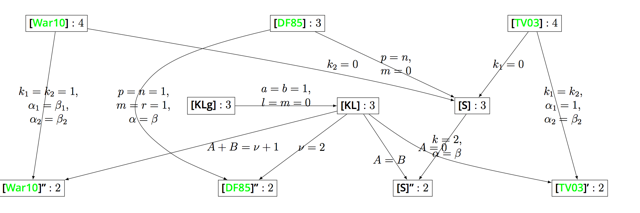
\includegraphics{../../fortexmacs/intdep.jpg}}
      \scalebox{0.2}{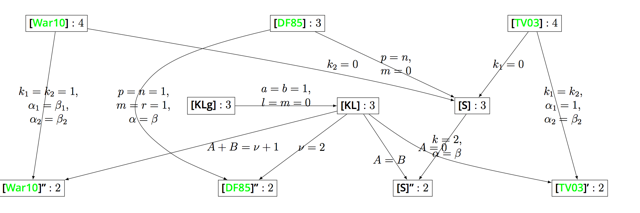
\includegraphics{../../fortexmacs/intdep.jpg}}
  \end{tabular}
  \caption{Hierarchy of various integral formul{\ae}\label{table}}
\end{table}

\begin{thebibliography}{1}
  \bibitem[1]{andrews2000special}G.~E.~Andrews, R.~Askey , and 
  R.~Roy.{\newblock} \tmtextit{Special Functions},  of \tmtextit{Encyclopedia
  of Mathematics and its Applications}, vol. 71.{\newblock} Cambridge
  University Press, Cambridge, 2000.{\newblock}
  
  \bibitem[2]{dotsenko1985four}V.~S.~Dotsenko  and  V.~A.~Fateev.{\newblock}
  Four-point correlation functions and the operator algebra in 2D conformal
  invariant theories with central charge $c \leq 1$, \tmtextit{Nuclear Phys.
  B}, vol. 251, pages 691--734, 1985.{\newblock}
  
  \bibitem[3]{forrester2008importance}P.~Forrester  and 
  S.~O.~Warnaar.{\newblock} The importance of the Selberg integral.{\newblock}
  \tmtextit{Bull. Amer. Math. Soc.}, vol. 45, no. 4, pages 489--534,
  2008.{\newblock} Available online at
  \url{https://doi.org/10.1090/S0273-0979-08-01221-4}.{\newblock}
  
  \bibitem[4]{kobayashi2011schrodinger}T.~Kobayashi  and  G.~Mano.{\newblock}
  \tmtextit{The Schr{\"o}dinger Model for the Minimal Representation of the
  Indefinite Orthogonal Group $O (p, q)$}.{\newblock} Memoirs of Amer. Math.
  Soc., vol. 213, no. 1000, 2011.{\newblock} Available online at
  \url{http://dx.doi.org/10.1090/S0065-9266-2011-00592-7}.{\newblock}
  
  \bibitem[5]{kobayashi2015symmetry}T.~Kobayashi  and  B.~Speh.{\newblock}
  \tmtextit{Symmetry Breaking for Representations of Rank One Orthogonal
  Groups}, {\newblock} \tmtextrm{\tmtextup{\tmtextmd{Memoirs of the Amer.
  Math. Soc.}}}, vol. \tmtextbf{238}. 2015.{\newblock} Available online at
  \url{http://dx.doi.org/10.1090/memo/1126}.{\newblock}
  
  \bibitem[6]{mehta2004random}M.~L.~Mehta.{\newblock} \tmtextit{Random
  matrices}, \tmtextit{\tmtextrm{\tmtextup{\tmtextmd{Pure Appl. Math., vol.
  142}}}}.{\newblock} Elsevier/Academic Press, Amsterdam, 2004.{\newblock}
  
  \bibitem[7]{Selberg:411367}A.~Selberg.{\newblock} Remarks on a multiple
  integral.{\newblock} \tmtextit{Norsk Mat. \doubt{1$\sim$} Tidsskr.}, vol. 26, pages 71--78,
  1944.{\newblock}
  
  \bibitem[8]{tarasov2003selberg}V.~Tarasov  and  A.~Varchenko.{\newblock}
  Selberg-type integrals associated with $\mathfrak{s}\mathfrak{l}_3$.{\newblock}
  \tmtextit{Lett. Math. Phys.}, vol. 65, no. 3, pages 173--185,
  2003.{\newblock} Available online at
  \url{http://dx.doi.org/10.1023/B:MATH.0000010712.67685.9d}.{\newblock}
  
  \bibitem[9]{warnaar2010sl3}S.~O.~Warnaar.{\newblock} The $\mathfrak{sl}_3$
  Selberg integral.{\newblock} \tmtextit{Adv. Math.}, vol. 224, no. 2, pages
  499--524, 2010.{\newblock} Available online at
  \url{http://dx.doi.org/10.1016/j.aim.2009.11.011}.{\newblock}
\end{thebibliography}

\end{document}
